\documentclass[tikz,border=8pt]{standalone}
% Shared look for every TikZ diagram. Load with % Shared look for every TikZ diagram. Load with % Shared look for every TikZ diagram. Load with \input{../../tools/tikz-style.tex}
\usepackage[T1]{fontenc}
\usepackage{lmodern}
\renewcommand{\sfdefault}{lmr}  % diagrams use the same serif as the text
\usetikzlibrary{arrows.meta, positioning, shapes.geometric, calc, fit, backgrounds}
\definecolor{cblue}{HTML}{4C78A8}
\definecolor{corange}{HTML}{F58518}
\definecolor{cgreen}{HTML}{54A24B}
\definecolor{cred}{HTML}{E45756}
\definecolor{cpurple}{HTML}{B279A2}
\definecolor{cgrey}{HTML}{6B6B6B}
\tikzset{
  every picture/.style={font=\sffamily, line width=1.2pt},
  box/.style={draw=#1, fill=#1!12, rounded corners=4pt, align=center, inner sep=7pt, minimum height=1.1cm},
  box/.default=cgrey,
  arrow/.style={-{Stealth[length=3mm]}, draw=cgrey, line width=1.4pt},
  title/.style={font=\sffamily\bfseries\Large},
  note/.style={font=\sffamily\small, text=cgrey, align=center},
}
\AtBeginDocument{\hyphenpenalty=10000 \exhyphenpenalty=10000}

\usepackage[T1]{fontenc}
\usepackage{lmodern}
\renewcommand{\sfdefault}{lmr}  % diagrams use the same serif as the text
\usetikzlibrary{arrows.meta, positioning, shapes.geometric, calc, fit, backgrounds}
\definecolor{cblue}{HTML}{4C78A8}
\definecolor{corange}{HTML}{F58518}
\definecolor{cgreen}{HTML}{54A24B}
\definecolor{cred}{HTML}{E45756}
\definecolor{cpurple}{HTML}{B279A2}
\definecolor{cgrey}{HTML}{6B6B6B}
\tikzset{
  every picture/.style={font=\sffamily, line width=1.2pt},
  box/.style={draw=#1, fill=#1!12, rounded corners=4pt, align=center, inner sep=7pt, minimum height=1.1cm},
  box/.default=cgrey,
  arrow/.style={-{Stealth[length=3mm]}, draw=cgrey, line width=1.4pt},
  title/.style={font=\sffamily\bfseries\Large},
  note/.style={font=\sffamily\small, text=cgrey, align=center},
}
\AtBeginDocument{\hyphenpenalty=10000 \exhyphenpenalty=10000}

\usepackage[T1]{fontenc}
\usepackage{lmodern}
\renewcommand{\sfdefault}{lmr}  % diagrams use the same serif as the text
\usetikzlibrary{arrows.meta, positioning, shapes.geometric, calc, fit, backgrounds}
\definecolor{cblue}{HTML}{4C78A8}
\definecolor{corange}{HTML}{F58518}
\definecolor{cgreen}{HTML}{54A24B}
\definecolor{cred}{HTML}{E45756}
\definecolor{cpurple}{HTML}{B279A2}
\definecolor{cgrey}{HTML}{6B6B6B}
\tikzset{
  every picture/.style={font=\sffamily, line width=1.2pt},
  box/.style={draw=#1, fill=#1!12, rounded corners=4pt, align=center, inner sep=7pt, minimum height=1.1cm},
  box/.default=cgrey,
  arrow/.style={-{Stealth[length=3mm]}, draw=cgrey, line width=1.4pt},
  title/.style={font=\sffamily\bfseries\Large},
  note/.style={font=\sffamily\small, text=cgrey, align=center},
}
\AtBeginDocument{\hyphenpenalty=10000 \exhyphenpenalty=10000}

\begin{document}
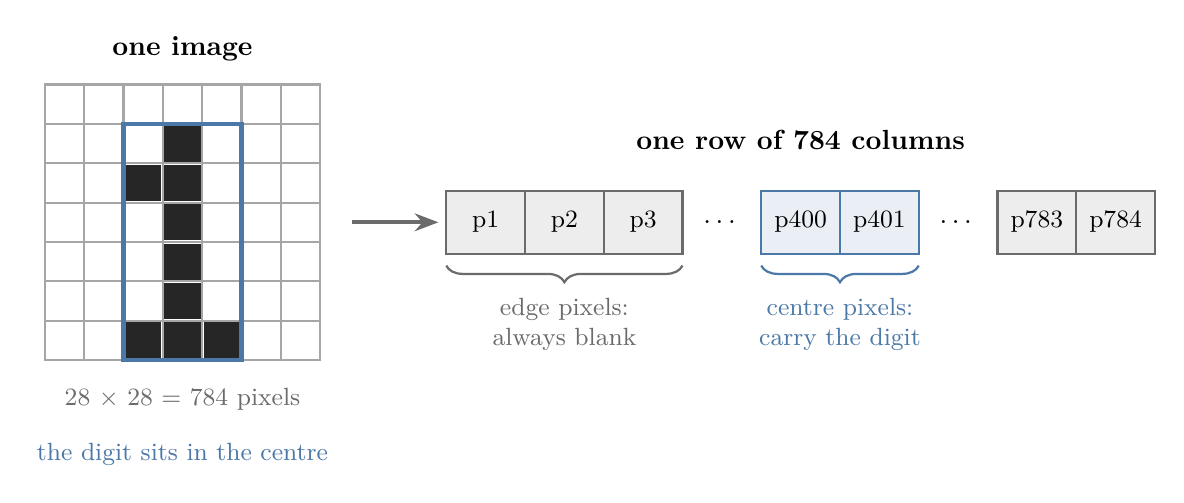
\begin{tikzpicture}[line width=0.8pt]
  % a small grid standing for the 28 x 28 image; dark cells draw a "1"
  \def\ink{{3/1,3/2,3/3,3/4,3/5,2/2,3/6,2/6,4/6}}
  \foreach \i in {0,...,6} \foreach \j in {0,...,6} {
    \draw[cgrey!60, fill=white] (\i*0.5, -\j*0.5) rectangle ++(0.5,-0.5);
  }
  \foreach \i/\j in {3/1,3/2,3/3,3/4,3/5,2/2,3/6,2/6,4/6}
    \fill[black!85] (\i*0.5+0.02, -\j*0.5-0.02) rectangle ++(0.46,-0.46);
  \draw[cblue, line width=1.6pt] (1.0,-0.5) rectangle (2.5,-3.5);
  \node[font=\sffamily\bfseries] at (1.75,0.45) {one image};
  \node[note] at (1.75,-4.0) {28 $\times$ 28 = 784 pixels};
  \node[note, text=cblue, align=center] at (1.75,-4.7) {the digit sits in the centre};
  % the same image as one table row
  \draw[arrow] (3.9,-1.75) -- (5.0,-1.75);
  \foreach \k/\t/\c in {0/p1/cgrey, 1/p2/cgrey, 2/p3/cgrey, 4/p400/cblue, 5/p401/cblue, 7/p783/cgrey, 8/p784/cgrey} {
    \node[draw=\c, fill=\c!12, minimum width=1.0cm, minimum height=0.8cm, font=\sffamily\small] at (5.6+\k*1.0,-1.75) {\t};
  }
  \node at (5.6+3*1.0,-1.75) {\dots};
  \node at (5.6+6*1.0,-1.75) {\dots};
  \node[font=\sffamily\bfseries] at (9.6,-0.7) {one row of 784 columns};
  \draw[decorate, decoration={brace, amplitude=6pt, mirror}, draw=cgrey] (5.1,-2.3) -- (8.1,-2.3)
    node[midway, below=8pt, note, align=center] {edge pixels:\\always blank};
  \draw[decorate, decoration={brace, amplitude=6pt, mirror}, draw=cblue] (9.1,-2.3) -- (11.1,-2.3)
    node[midway, below=8pt, note, text=cblue, align=center] {centre pixels:\\carry the digit};
\end{tikzpicture}
\end{document}
